\documentclass[journal]{IEEEtran}

\usepackage{graphicx}
\usepackage{amsmath,amssymb}
\usepackage{hyperref}
\usepackage{float}
\usepackage{subcaption}
\usepackage{booktabs}
\usepackage{pgfplotstable}
\usepackage{siunitx}
\usepackage{qrcode}

\pgfplotstableset{
    col sep=comma,
    every head row/.style={before row=\toprule, after row=\midrule},
    every last row/.style={after row=\bottomrule},
}

\title{Anomaly Detection on the LHC Olympics 2020 Dataset: A Reproducible Baseline and Particle-Transformer Extensions}

% NOTE: Fill in author/affiliation details.
\author{\IEEEauthorblockN{\textit{(Author Name)}}\\
\IEEEauthorblockA{\textit{Istanbul University, DAMLA LAB}\\}}

\begin{document}
\maketitle

\begin{abstract}
This report documents an end-to-end machine learning pipeline for anomaly detection in high-energy physics collider events, implemented for the LHC Olympics 2020 benchmark. A reproducible baseline (autoencoder and MLP classifier) is provided alongside Particle Transformer (ParT) variants for particle-based representations. The repository includes data loaders for both processed feature matrices (\texttt{.npz}) and raw LHCO-style HDF5 files (\texttt{.h5}), training with checkpointing, and evaluation utilities producing anomaly-score distributions, ROC curves (when labels are available), and a simple bump-hunt significance estimate. Representative results are reported for both synthetic labeled validation data and a background-only processed dataset.
\end{abstract}

\begin{IEEEkeywords}
Anomaly detection, autoencoder, Particle Transformer, high-energy physics, LHC Olympics 2020, reproducibility.
\end{IEEEkeywords}

\section{Introduction}
Unsupervised and weakly supervised anomaly detection methods are widely studied for discovering rare or unexpected signatures in particle physics. The LHC Olympics 2020 benchmark provides standardized datasets and evaluation conventions to compare approaches under realistic constraints. This project implements a compact, reproducible pipeline that supports rapid iteration from baseline feature-based models to particle-based transformer architectures.

The objective is twofold: (i) to provide a clean, runnable reference implementation (data loading, training, evaluation, and plotting), and (ii) to serve as a scaffold for extending to Particle Transformer models suitable for jet/particle representations.

\section{Pipeline Overview}
Figure~\ref{fig:pipeline} summarizes the implemented pipeline. Data may be provided either as processed feature matrices (\texttt{.npz}) or as raw LHCO HDF5 files (\texttt{.h5}). Training produces checkpoints and logs. Evaluation generates diagnostic figures and summary metrics.

\begin{figure}[H]
\centering
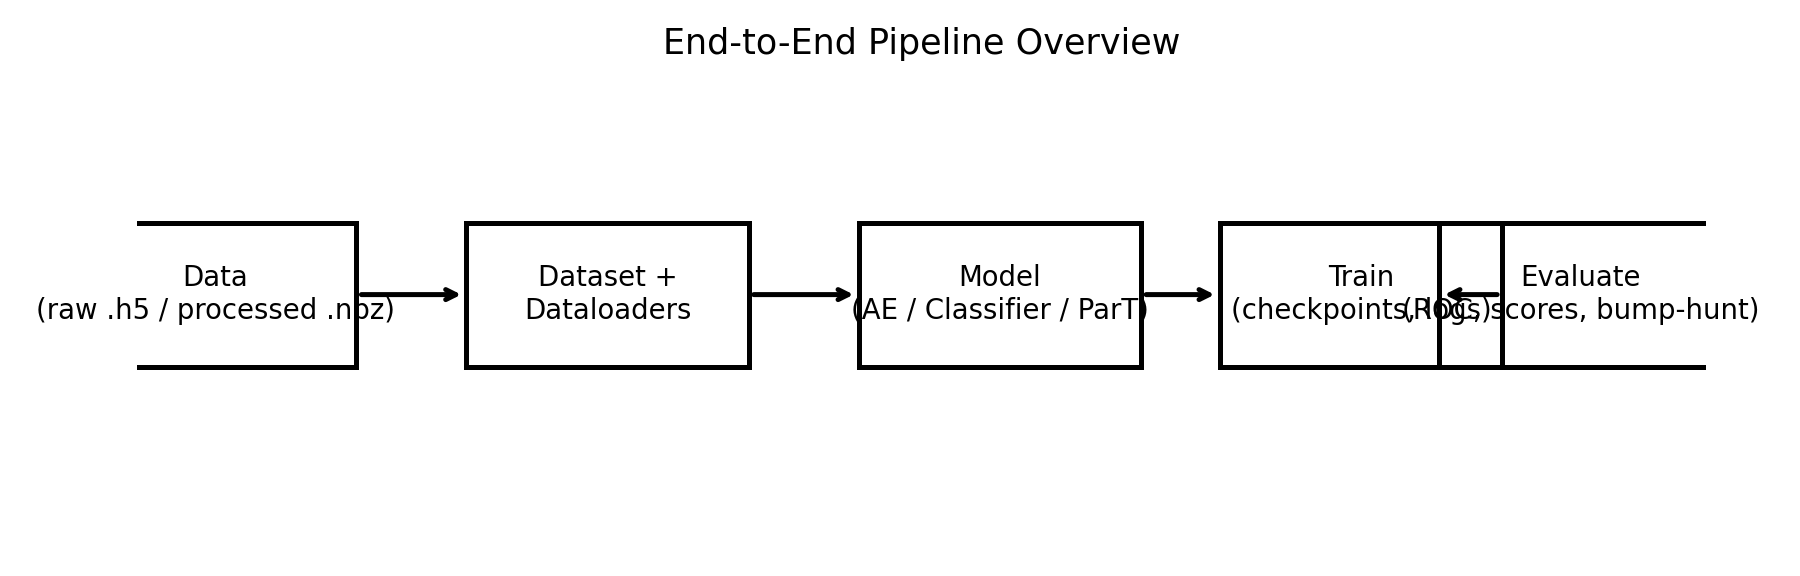
\includegraphics[width=\linewidth]{plots/pipeline.png}
\caption{End-to-end pipeline implemented in this repository.}
\label{fig:pipeline}
\end{figure}

\section{Data and Preprocessing}
\subsection{Supported file formats}
Two dataset pathways are supported:
\begin{itemize}
\item \textbf{Processed features (\texttt{.npz}).} A dense matrix $X\in\mathbb{R}^{N\times D}$ with optional labels $y\in\{0,1\}^N$.
\item \textbf{Raw LHCO HDF5 (\texttt{.h5}).} A pandas-style dataset located at \texttt{df/block0\_values}. Reading requires the Blosc filter plugin (\texttt{hdf5plugin}).
\end{itemize}

\subsection{Feature normalization}
For processed feature files, the stored mean/standard deviation can be used to normalize the inputs. In the included runs, the baseline models consume the feature dimension $D=128$.

\section{Models}
\subsection{Baseline autoencoder}
The baseline autoencoder maps $x\in\mathbb{R}^D$ to a latent vector $z\in\mathbb{R}^L$ and reconstructs $\hat{x}\in\mathbb{R}^D$. The anomaly score is the per-sample reconstruction error,
\begin{equation}
    s(x) = \frac{1}{D}\sum_{i=1}^{D}\left(\hat{x}_i - x_i\right)^2.
    \label{eq:ae_score}
\end{equation}

\subsection{Baseline classifier}
A simple MLP classifier predicts class logits for background vs. signal. For labeled datasets, ROC/AUC is computed from the predicted probability of the positive class.

\subsection{Particle Transformer extensions}
Particle Transformer (ParT) models are included for particle-based representations, enabling attention over particles and learned pairwise structure. Smoke tests verify that both ParT autoencoder and ParT classifier variants train end-to-end on small synthetic datasets.

\section{Training and Evaluation Protocol}
\subsection{Training}
Training uses Adam optimization with mean-squared error (autoencoder) or cross-entropy (classifier). Checkpoints are saved as \texttt{best\_model.pt} (lowest validation loss) and \texttt{final\_model.pt}. Loss logs are recorded per epoch.

\subsection{Evaluation}
Evaluation produces:
\begin{itemize}
\item anomaly-score (or classifier-score) distributions,
\item ROC curves and AUC when both classes are present,
\item a bump-hunt diagnostic using a polynomial background fit and a local-significance approximation.
\end{itemize}

\section{Results}
\subsection{Run summary}
Table~\ref{tab:results_summary} lists representative results from the executed runs in this workspace.

\begin{table}[H]
\centering
\caption{Summary of representative training/evaluation runs. AUC is reported only when both background and signal labels are present.}
\label{tab:results_summary}
\pgfplotstabletypeset[
    columns={run_id,dataset,model,auc,z_score,signal_count,background_estimate,notes},
    columns/run_id/.style={column name={Run}},
    columns/dataset/.style={column name={Dataset}},
    columns/model/.style={column name={Model}},
    columns/auc/.style={column name={AUC}},
    columns/z_score/.style={column name={$Z$}},
    columns/signal_count/.style={column name={Obs. (win)}},
    columns/background_estimate/.style={column name={Bkg. (win)}},
    columns/notes/.style={column name={Notes}, string type},
    every head row/.style={before row=\toprule, after row=\midrule},
    every last row/.style={after row=\bottomrule},
]{tables/results_summary.csv}
\end{table}

\subsection{Synthetic validation (baseline models)}
Figure~\ref{fig:ae_loss} and Figure~\ref{fig:clf_loss} show the training curves for short synthetic runs. The autoencoder achieved AUC $\approx 0.9903$ on the synthetic evaluation split, with clearly separated anomaly score distributions (Figure~\ref{fig:ae_scores}). The classifier achieved AUC $\approx 0.9616$ with score separation (Figure~\ref{fig:clf_scores}).

\begin{figure}[H]
\centering
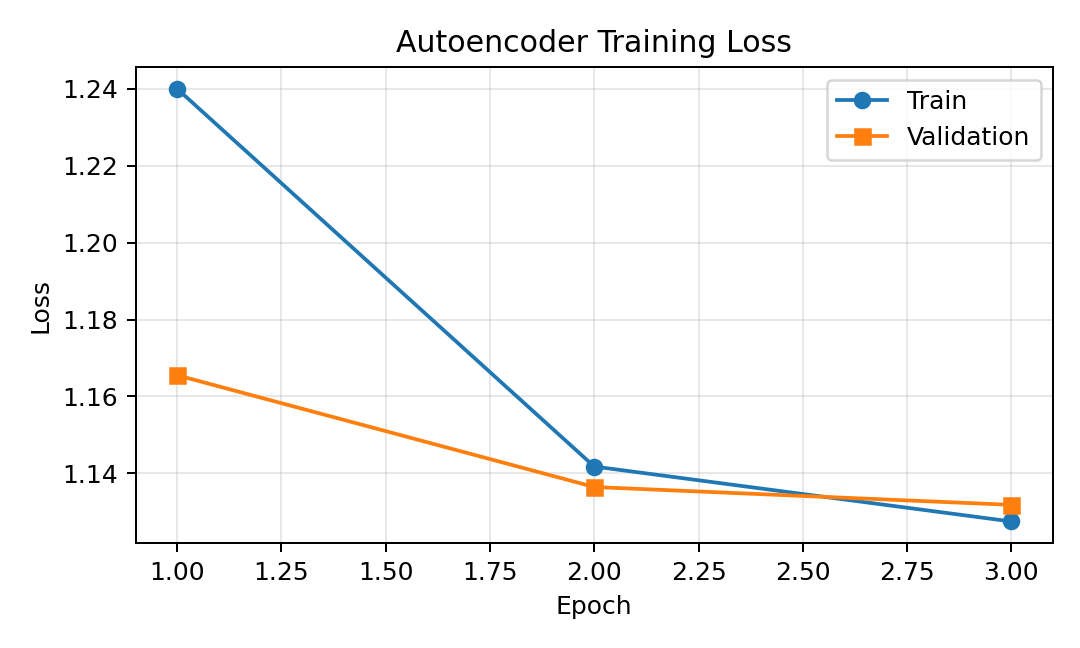
\includegraphics[width=0.95\linewidth]{plots/loss_autoencoder.png}
\caption{Baseline autoencoder training/validation loss (synthetic).}
\label{fig:ae_loss}
\end{figure}

\begin{figure}[H]
\centering
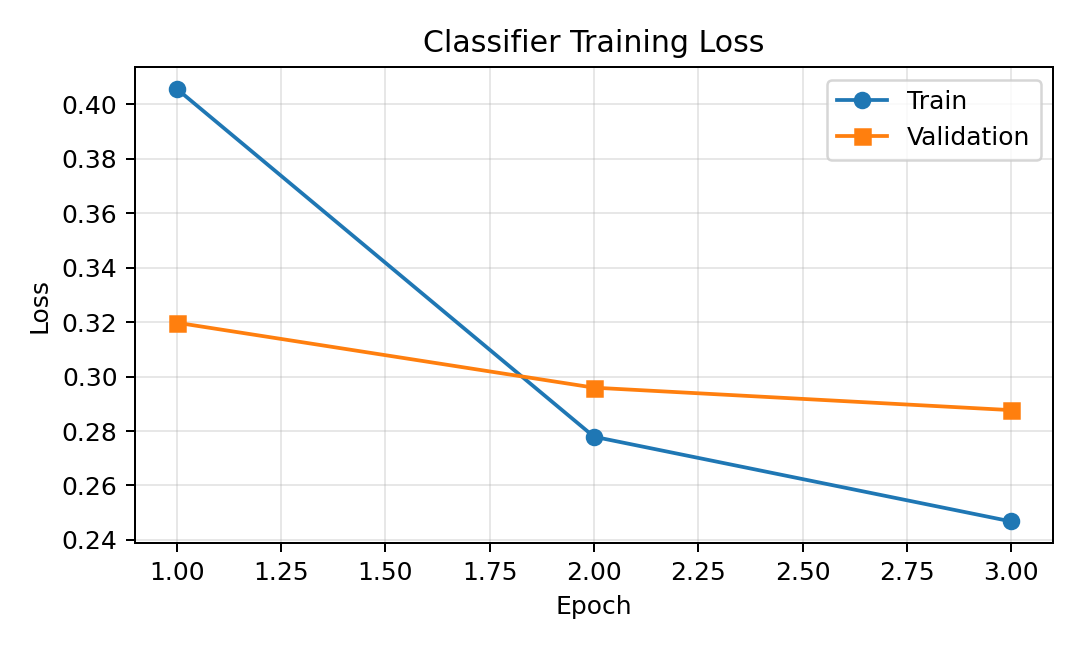
\includegraphics[width=0.95\linewidth]{plots/loss_classifier.png}
\caption{Baseline classifier training/validation loss (synthetic).}
\label{fig:clf_loss}
\end{figure}

\begin{figure}[H]
\centering
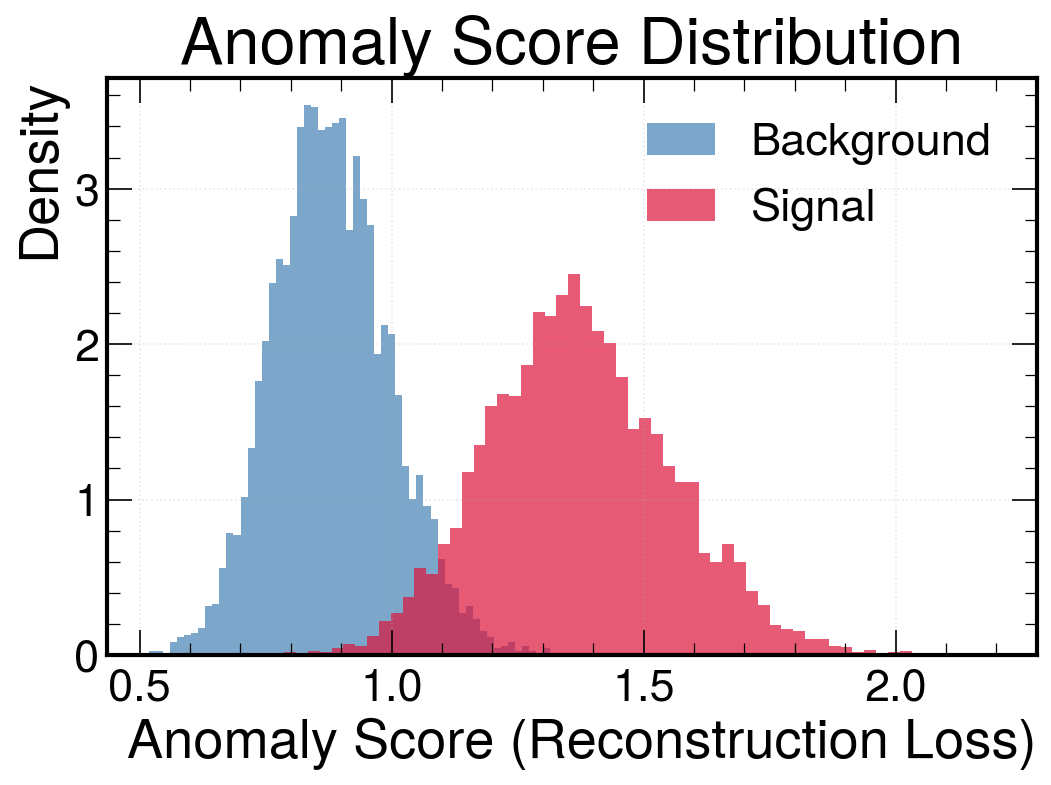
\includegraphics[width=\linewidth]{plots/ae_anomaly_scores.png}
\caption{Autoencoder anomaly-score distribution on synthetic evaluation data (background vs. signal).}
\label{fig:ae_scores}
\end{figure}

\begin{figure}[H]
\centering
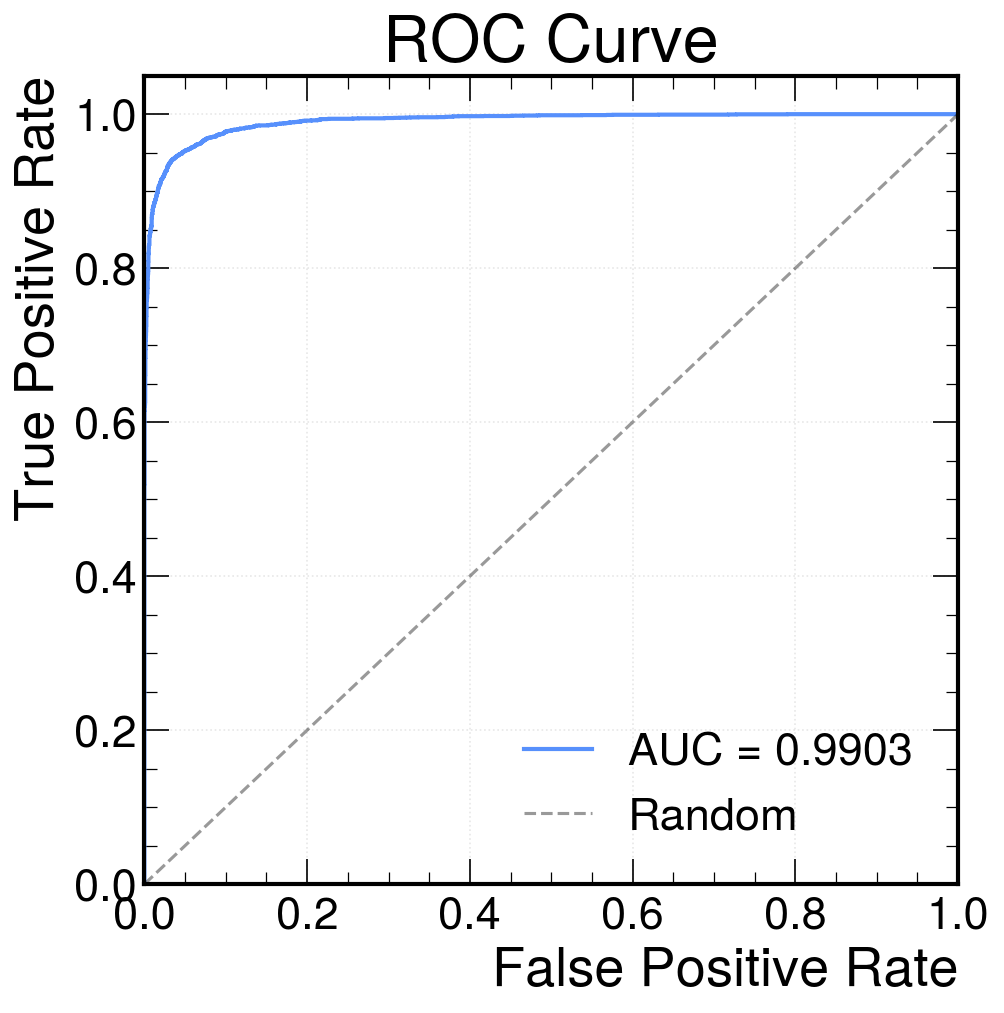
\includegraphics[width=\linewidth]{plots/ae_roc.png}
\caption{Autoencoder ROC curve on synthetic evaluation data.}
\label{fig:ae_roc}
\end{figure}

\begin{figure}[H]
\centering
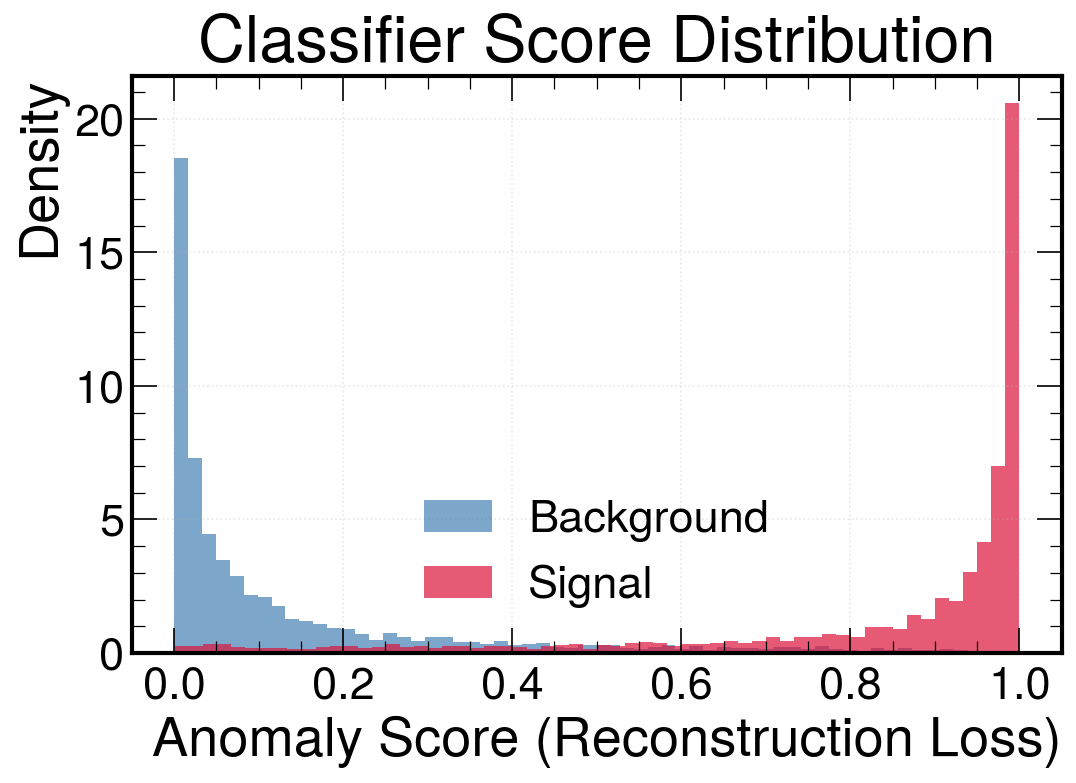
\includegraphics[width=\linewidth]{plots/clf_scores.png}
\caption{Classifier score distribution on synthetic evaluation data (background vs. signal).}
\label{fig:clf_scores}
\end{figure}

\begin{figure}[H]
\centering
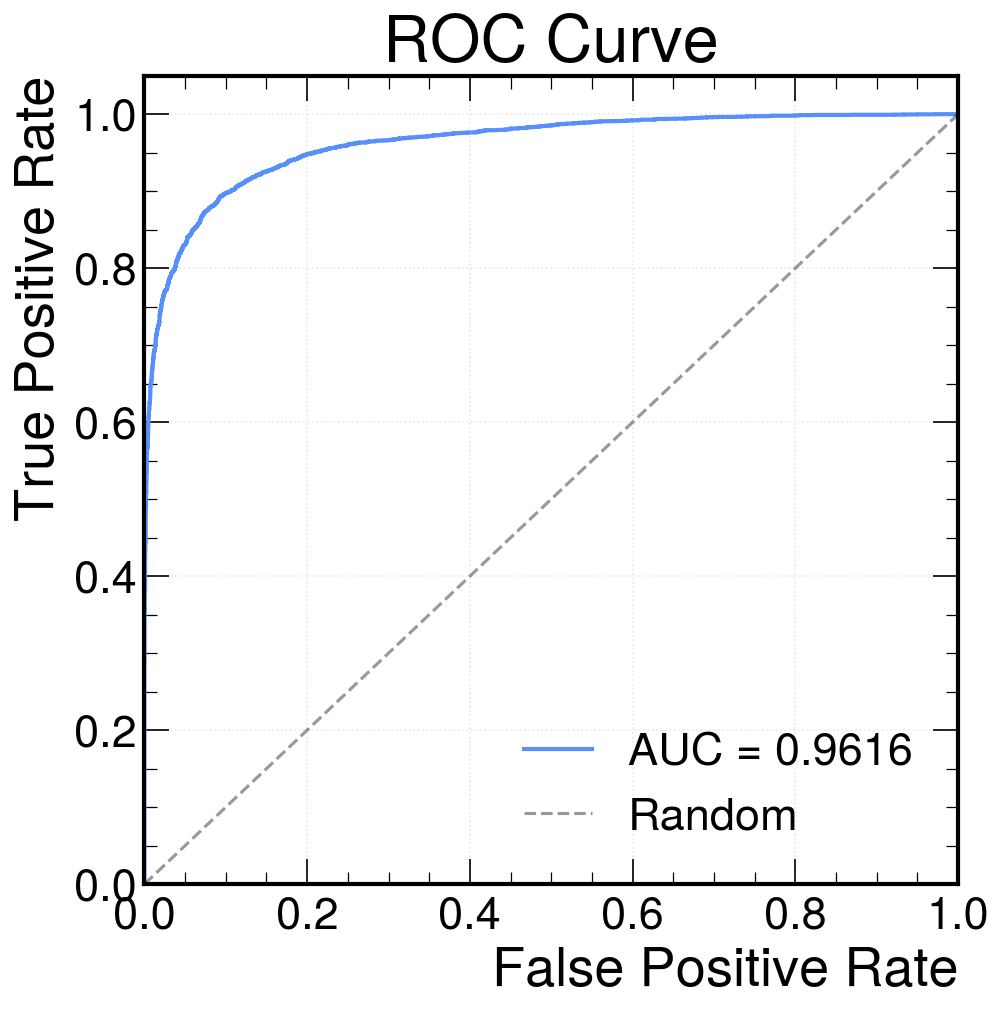
\includegraphics[width=\linewidth]{plots/clf_roc.png}
\caption{Classifier ROC curve on synthetic evaluation data.}
\label{fig:clf_roc}
\end{figure}

\subsection{Background-only processed dataset}
For the processed feature file \texttt{features\_K30\_events\_LHCO2020\_backgroundMC\_Pythia.npz}, labels contain only background events. In this case, ROC/AUC is undefined and is therefore skipped. Figure~\ref{fig:real_bg_scores} provides the anomaly-score distribution for qualitative inspection.

\begin{figure}[H]
\centering
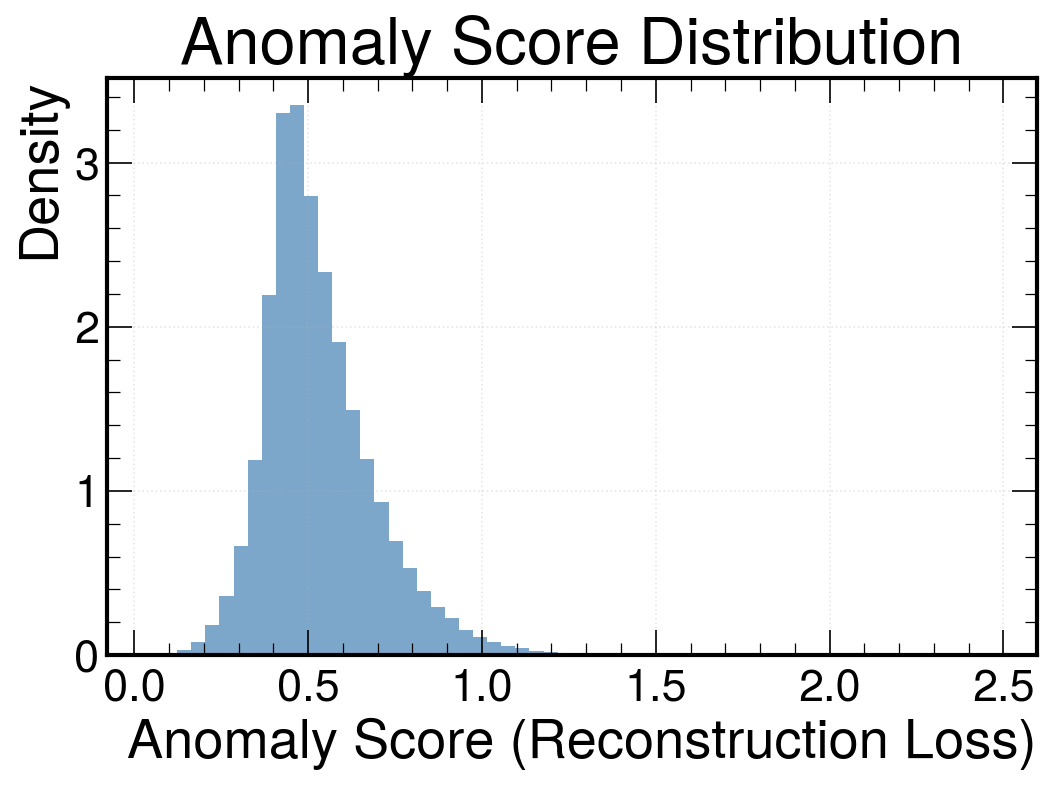
\includegraphics[width=\linewidth]{plots/real_bg_anomaly_scores.png}
\caption{Autoencoder anomaly-score distribution on the background-only processed dataset.}
\label{fig:real_bg_scores}
\end{figure}

\section{Discussion}
The baseline pipeline provides a reliable reference for experimentation. Synthetic results demonstrate that the evaluation stack (plots, ROC, and bump-hunt diagnostic) functions end-to-end and is sensitive to separable labeled distributions.

For real benchmark usage, two practical considerations are highlighted:
\begin{itemize}
\item \textbf{Label availability.} Many challenge scenarios are unlabeled or background-only at development time; ROC/AUC should be computed only when both classes are present.
\item \textbf{Bump-hunt interpretation.} The implemented bump-hunt routine is a simplified diagnostic. Its $Z$-scores should be treated as qualitative indicators unless the mass observable, window definition, and background model are validated for the target dataset.
\end{itemize}

ParT models are integrated and pass smoke tests; further work would focus on dataset representations (particle four-vectors, masking/padding conventions), hyperparameter sweeps, and robust physics-motivated evaluation.

\section{Conclusion}
A complete, runnable anomaly-detection pipeline for the LHC Olympics 2020 ecosystem is implemented, spanning data loading, baseline and transformer-based models, training with checkpointing, and evaluation with consistent plots and diagnostics. The project is suitable as a reproducible baseline and as a foundation for more physics-realistic ParT-based anomaly detection studies.

\section{Additional Resources}
% NOTE: Replace the URL with your repository link if available.
\noindent\textbf{Repository (local):} \texttt{C:\\Users\\Pc\\Desktop\\LOCALS\\DAMLALAB\\ML\_projects\\LHC\_olympics}\\
\noindent\textbf{Repository URL (optional):} \url{\textit{(insert URL here)}}\\
\vspace{4pt}
\noindent\textbf{QR Code:}\\
\qrcode[height=1in]{C:\\Users\\Pc\\Desktop\\LOCALS\\DAMLALAB\\ML\_projects\\LHC\_olympics}

\begin{thebibliography}{9}
\bibitem{lhco2020}
The LHC Olympics 2020 Challenge, benchmark datasets and documentation (project context).

\bibitem{part}
H. Qu and L. Gouskos, ``Jet tagging via Particle Transformer,'' arXiv:2202.03772.
\end{thebibliography}

\end{document}
